\documentclass[runningheads]{llncs}

% \documentclass{article}

\usepackage[
backend=biber,
style=alphabetic,
]{biblatex}

\usepackage{mathpartir}
\usepackage{hyperref}
\usepackage{mathtools}
\usepackage{stmaryrd}
\usepackage{listings}

\usepackage{graphicx}
\graphicspath{ {./images/} }


\makeatletter % allow us to mention @-commands
\def\arcr{\@arraycr}
\makeatother

\lstset{
    % identifierstyle=\color{violet},
    % textcolor=blue,
    % keywordstyle=\color{blue},
    keywordstyle=\text,
    basicstyle=\ttfamily,
    mathescape=true,
    showspaces=false,
    morekeywords={let, fix, in}
}
\usepackage[utf8]{inputenc}
% \usepackage[T1]{fontenc}


\title{Synthesis of stochastic programs from data}
\author{Thomas Logan}
\institute{University of Texas at Austin}

\begin{document}

\maketitle

\section{Introduction}
The aim of this project is to automatically synthesize  programs from data sets. 
The intended scenario consists of a user who wants to fit a line to some data.
It is quite easy to encode an equation
from inputs to outputs in a typical programming language, such as the following:
\[ f(x) = m x + b \] 

However, current programming languages do not provide a compact notation 
for representing the requirement that the weights $m$ and $b$ are learned from data.
\textit{Pyro} \cite{} is a language embedded in \textit{Python} \cite{} for 
expressing the requirements of learning weights from data 
with probabilities for measuring uncertainty in the learned result. 
In Pyro, the simplest way to represent the above linear equation is as follows: 

\begin{lstlisting}[language=Python]
def model(xs, ys=None):
    m = pyro.param("m", torch.tensor(0.))
    b = pyro.param("b", torch.tensor(0.))
    
    with pyro.plate("data", len(xs)):
        return pyro.sample("ys", 
            dist.Normal(m * xs + b, 1.), obs=ys)
\end{lstlisting}

Clearly, there is a vast increase in notational noise, within which the essence of the idea is buried. 

To reduce the notational noise, this project introduces a simple programming language 
that allows expressing learnable models in a succinct notation. In this new language,
we can express a model for learning a linear equation as follows: 

\begin{lstlisting}[language=Python]
x => {y | x, y : data}
    m $\sim$ normal(0., 1.); 
    b $\sim$ normal(0., 1.); 
    normal(m * x + b, 1)
\end{lstlisting}

The notation of our new language is is far more compact than Pyro's. 
It is only slightly more complicated than the bare linear equation, which is
due to annotating information about prior beliefs on the weights, the data, and 
distribution of the data in relation to the equation. 

Unfortunately, this solution leaves open another problem. How do we conjure up some 
initial belief about the distributions and the shape of the equation? 

To avoid needing to specify these details, we simplify the specification further, such that the 
user can simply state the data and its relation to inputs and outputs. 

\begin{lstlisting}[language=Python]
x => {y | x, y : data}
\end{lstlisting}

The first part of the solution compiles a program in the DSL into a Pyro model and applies Pyro's 
\textit{stochastic variational inference} (SVI) algorithm \cite{} to learn posterior distributions for the weights. 

The second part of the solution encodes the DSL grammar and semantics into
an logical formula in Z3 \cite{} and uses Z3's \textit{satisfiability modulo theories} (SMT) \cite{} algorithm to search
for a program with priors.  
The particular technique for constructing the search space from the grammar and semantics 
is based on that of Ellis et al \cite{}.
Unfortunately, at the time of this writing, Z3 does not terminate in a reasonable amount of time, 
despite using an encoding very similar to that of Ellis et al. 
After finding the program, the first part may be used to learn posteriors. 

\section{Language}

The programs in the domain specific language are constructed using the following syntax:

\[
  \begin{array}{l @{} l}
    f &{} ::= p \Rightarrow s\ b \\
    s &{} ::= \{ x \ |\ p : \text{data} \} \\
    p &{} ::= x  \ |\ x,\ p \\
    b &{} ::= x\ \sim\ d\ ;\ b \ |\ x\ \#\ n\ \sim\ d\ ;\ b \ |\ d \\ 
    d &{} ::= 
        \text{normal}(e, e) \ |\ 
        \text{lognorm}(e, e) \ |\ 
        \text{uniform}(e, e) \ |\ 
        \text{halfnorm}(e) \ |\ 
        @(e) \\ 
    e &{} ::= q\ \vec{r} \\
    r &{} ::= +\ q \ |\ -\ q \\
    q &{} ::= a\ \vec{z} \\
    z &{} ::= *\ q \ |\ /\ q \\
    a &{} ::= (e) \ |\ \text{mean}(x) \ |\ \text{align}(x)\\
  \end{array}
\]
.

To see what these combinations of syntax mean, consider a program
for predicting the the number of unemployment insurance claims 
between the 2008 recession and the 2020 pandemic \cite{}.
Let's examine the plot of the data to gauge its shape.
\newline
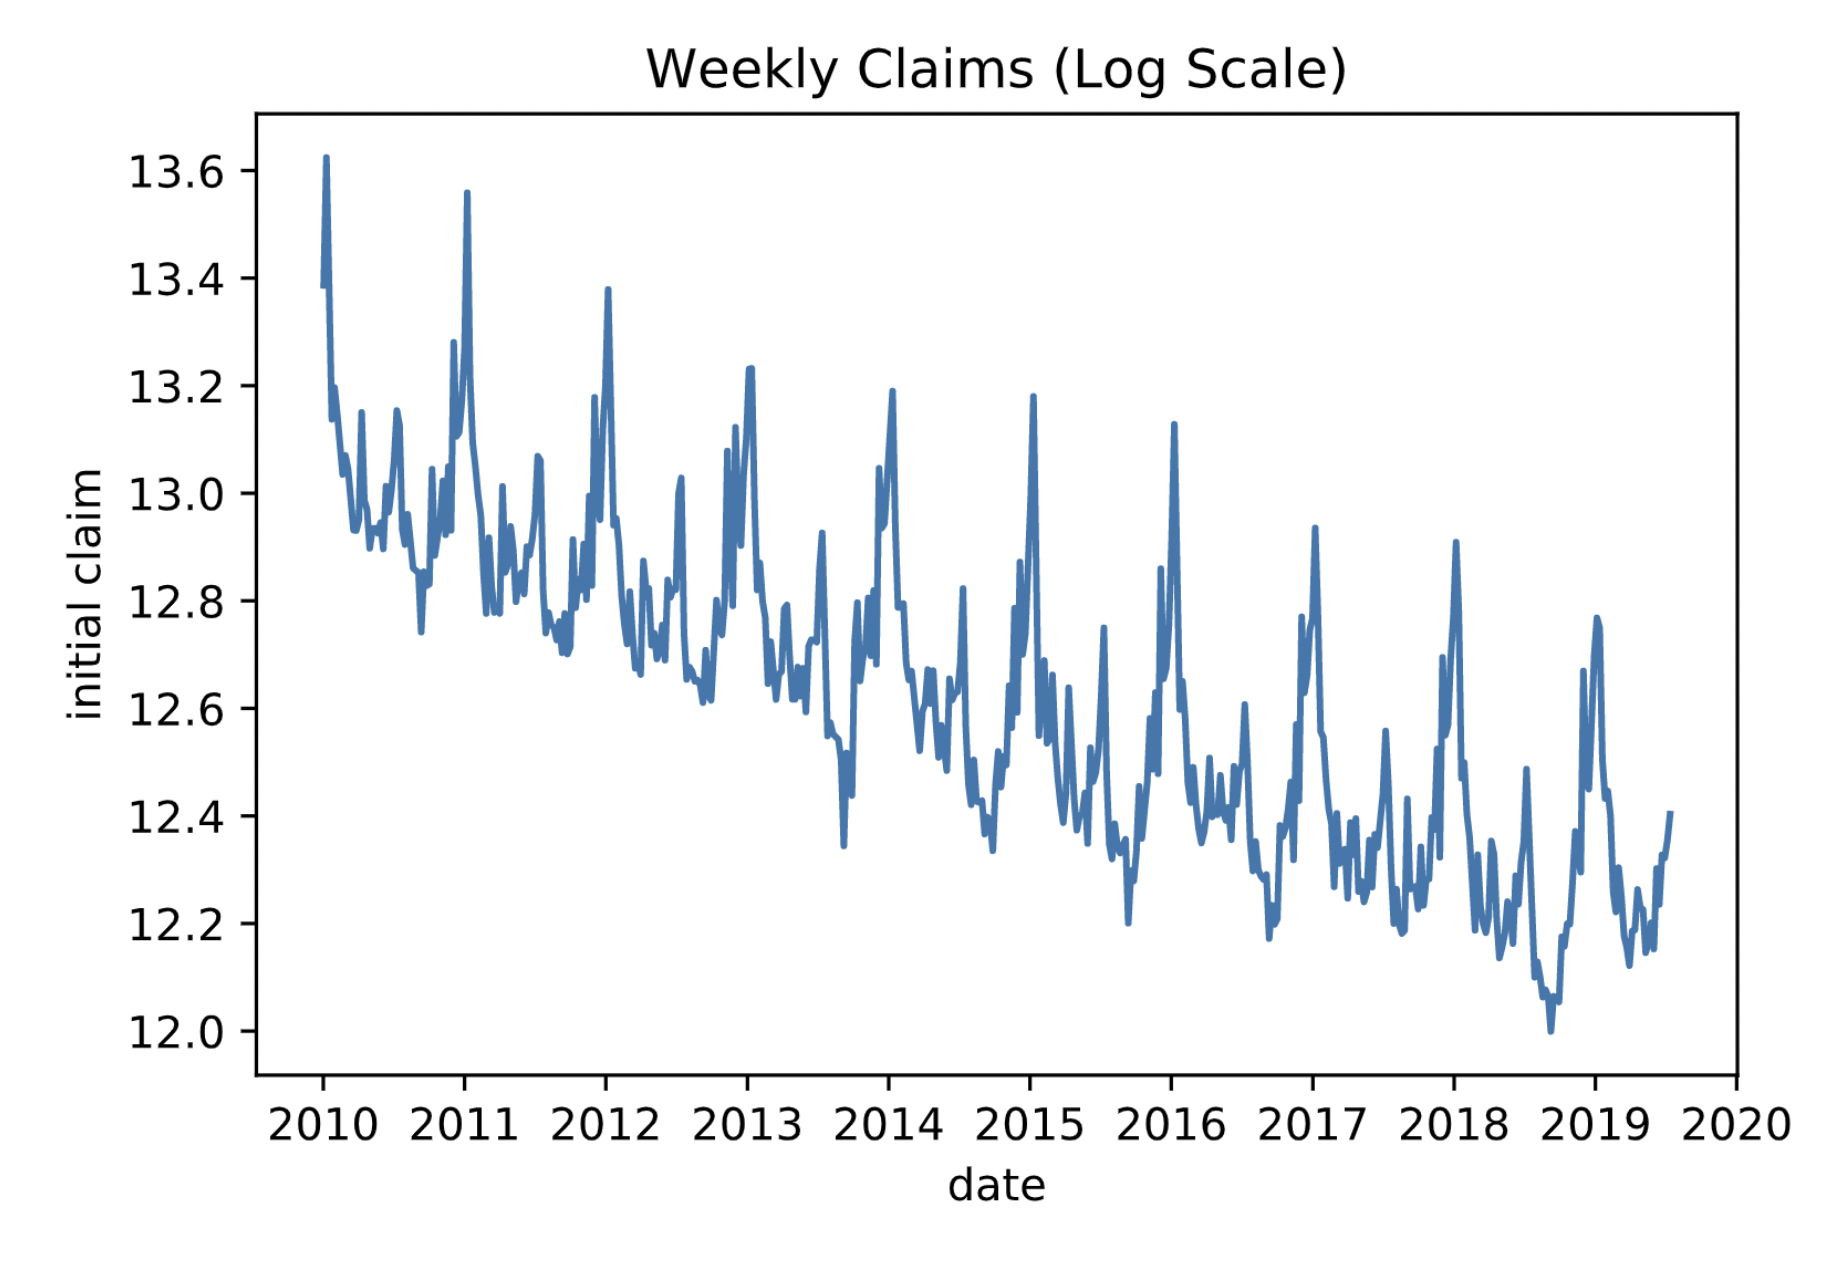
\includegraphics[scale=0.35]{weekly_claims}

There appears to be an overall trend that's fairly linear with respect to the year. 
However, there are also periodic trends that seem to depend on the time of year.  
We can capture these trends with the following program:

\begin{lstlisting}[language=Python]
t => {n | t, n : data}
    m $\sim$ normal(0., 1.); 
    osd $\sim$ halfnorm(1.); 
    bs $\#$ 52 $\sim$ normal(0., 1.); 
    bs $\sim$ @(bs - mean(bs));
    lognorm(m * t + align(bs), osd)
\end{lstlisting}

The program represents a function from a weekly time index to a number of claims.
The parameter $t$ represents a single input. The variable $n$ represents
the ouput, such that the first column of the data are used as inputs, 
and second column of the data are observed outputs.
The rest of the program is the body of the function.
First it samples a slope $m$ from a normal distribution centered at 0 with 
a standard deviation of 1. To handle the periodic trends, it constructs
a plate $bs$ of 52 independent elements, where each is sampled from 
a normal distribution. In order to ensure the weight $m$ governs
the overall trend, we need the values of $bs$ to cancel each other out.
To this end, the program recomputes the values of the vector point-wise 
by subtracting the mean from the original value. The notation $@$ simply indicates
to use the value of the expression directly.
The resulting number of claims is drawn from a log normal distribution
governed by $m * t + \text{align}(bs)$. The term $\text{align}(bs)$ takes an element from $bs$ 
at an implicit iteration index modulo 52. 



\section{Compiling programs into Pyro}
In order to learn the posterior distributions of our programs, we compile down into  
a Pyro model and run Pyro's SVI algorithm. For the most part, the compilation technique
is fairly standard, but the $\text{align}(\cdot)$ operator deserves special attention. 
Pyro's model operates over tensors of data, while the program DSL operates over points. 
This difference beomes noticeable when compiling the indexing operation. Pyro is
operating over tensors that are computed via data-parallelism. There is no
equivalent data-parallel operation for indexing a matrix with a vector of indices.
Thus, indexing is actually compiled into repeating the target plate and aligns lengthens it
to match the size of the implicit number of total iterations.    
The example of unemployment insurance claims above is compiled into the following model.

\begin{lstlisting}[language=Python]
def model(t, n=None):
    m = pyro.sample("m", dist.Normal(0.0, 1.0))
    osd = pyro.sample("osd", dist.HalfNormal(1.0))
    with pyro.plate("bs_plate", 52):
        bs = pyro.sample("bs", dist.Normal(0.0, 1.0))
    bs = bs - bs.mean()
    with pyro.plate("data", len(t)):
        return pyro.sample("n", dist.Normal(
            m * t + bs.repeat(math.ceil(len(t)/len(bs)))
                [:len(t)], osd), obs=n)
\end{lstlisting}


\section{Encoding language into Z3}
In order to search for viable programs, we encode the language's syntax and semantics, 
along with the input data into a Z3 formula and run Z3's SMT algorithm.
The technique for encoding a space of programs is far more intricate than compiling a program.

It constructs a search space recursively by following the structure of the grammar. 
If the syntax allows a choice of productions, it constructs a boolean control variable for each choice
and constructs a an if-then-else term across each choice's abstract value, guarded its respective control variable. 
Additionally, it constructs the constraint that at most one control variable for a particular set of choices    
is allowed to be true, which along with the if-then-else constraint, ensures
that exactly one subterm for each choice is identified, if there is a solution.  

The encoding specifies how leaf terms are denoted as Z3 formulas for each sample input.
The leaf syntax representing a parameter simply denotes a the corresponding column of the input data. 
The denotation may be abstract consisting of both a Z3 expression and a constraint on that expression. 
The formulas of subterm are propagated up to larger composite terms according to the semantics of 
the composite terms.



\end{document}